\section{Moonpig}~\label{study-moonpig}
Moonpig is an e-commerce business in Europe that sells greeting cards and related gifts online; they operate in the United Kingdom, USA and Australia. They have a highly rated mobile app, with overall ratings of 4.8/5 in Google Play and the Apple App Store. Note some portions of this case study were published in \citep{harty_better_android_apps_using_android_vitals}.

{\renewcommand{\arraystretch}{0.8}% Tighter
\begin{table}[htbp!]
    \centering
    \small
    \setlength{\tabcolsep}{1pt}
    \begin{tabular}{ll}
       % Question &Answer  \\
       \toprule
       Website &\url{https://www.moonpig.com/uk/} \\
       Founded &2000 \\
       Business Domain & Greeting cards and gifts \\
       Business type & e-commerce \\
       Technologies  & Native apps, Robospice, \\
       & AWS, GraphQL, nodeJS, \\
       & Commercetools, ContentStack, ... \\
       Source code  &Closed and not available for research \\
       Analytics used by team &Firebase, Google Play Console \\
       Development Practices & High performance engineering, ATDD, \\
         & micro-services architecture \\
       \midrule
       User base &100,000's for the Android app\\
       Installations &1,000,000+ for the Android app\\
       \midrule
       Research methods &In person interviews, email discussions, remote testing \\
       Analytics collected &Google Play Console with Android Vitals \\
       Research software &They used Vitals-Scraper, otherwise none applicable.\\
       Additional data collected &Interview notes and emails \\
       Active period &June 2019 to July 2019, with updates in Oct 2019 and Feb 2020. \\
       \bottomrule
    \end{tabular}
    \caption{Case Study key facts: Moonpig}
    \label{tab:moonpig_anaytics_overview}
\end{table}
}

\begin{comment}
Sources: 
- 4.8 rating in Apple App Store https://apps.apple.com/app/id393730279
- 4.8 rating in Google Play, and install count  https://play.google.com/store/apps/details?id=com.commonagency.moonpig.uk
- ATDD https://medium.com/moonpigtech/the-android-testing-approach-part-1-atdd-6e26e3851c08
- High Performance Engineering https://medium.com/moonpigtech/working-remotely-as-a-high-performance-engineering-team-at-moonpig-957b267de1d4
- micro services (in 2020) https://medium.com/moonpigtech/introducing-the-moonpig-engineering-blog-c3fde37f06bd
- Robospice - email discussions and Android Vitals crash reports
\end{comment}



\subsection{Moonpig: Background - How the case study came about}
One of the developers of the Android app learned about this research and offered to provide their insights into their use of mobile analytics for their Android app. Both the head of engineering and communication manager approved him doing so and gave permission for the material to be used.

\subsection{Moonpig: development microcosm}
The engineering organisation consisted of various teams, including a team for the Android app. At the time of the case study, the Android app combined several generations of their architecture and used various third-party libraries.

Their software engineering team have been actively involved in encouraging the wider software engineering community to learn and practice good software development practices, for example by hosting Coding DoJos~\footnote{Historical examples available online on twitter \url{https://mobile.twitter.com/moonpigtech} and in a \href{https://www.codurance.com/publications/newsletters/2020-02-13-newsletter}{Codurance newsletter} from February 2020, for example.}. They practiced similar software development practices when developing their production software.

\subsection{Moonpig: Experiences of using mobile analytics}
The development team use Firebase Crashlytics and Google Analytics for diagnostics in addition to the information available in Android Vitals; and estimated they used Android Vitals approximately 30\% of their time to identify flaws and issues related to their Android app.
%
They also incorporated in-app analytics by using Firebase Analytics which recorded analytics related to how the users use the mobile apps and whether errors or other problems occurred while the app was being used. 

\definecolor{Gray}{gray}{0.85}

\begin{table}
  \begin{threeparttable}
  % \begin{tabular}{ccccccR{2cm}}
  \caption{July 2019 Case Studies: Comparisons of sessions impacted by crashes}
  \label{tab:July2019_case_studies_apps_crash_rate}
  \begin{tabular}{>{\centering\arraybackslash}m{0.5cm}>{\centering\arraybackslash}m{0.5cm}>{\centering\arraybackslash}m{0.5cm}>{\centering\arraybackslash}m{0.5cm}>{\centering\arraybackslash}m{0.6cm}|>{\centering\arraybackslash\columncolor{Gray}}m{0.8cm}|>{\raggedright\arraybackslash}m{2.6cm}}
    \toprule
     \multicolumn{5}{c}{Android Version} &Overall& \\
    6.0.1 &7 &8 &8.1 &9 &Crashes &App\\
    \midrule
    0.42\% &1.43\% &3.48\% &3.48\% &6.49\% &4.05\% &Kiwix\tnote{1}\\
           &0.45\% &0.75\% &0.89\% &1.52\% &1.07\% &WikiMed (en)\tnote{2}\\
           &       &2.69\% &4.07\% &3.77\% &3.45\% &PhET Simulations\tnote{3}\\
           &       &       &0.22\% &0.15\% &0.19\% &Moodspace\tnote{4} \\
           &0.06\% &0.14\% &0.09\% &0.93\% &0.61\% &Moonpig\tnote{5}\\
           &       &1.38\% &1.51\% &2.16\% &1.66\% &Pocket Paint\tnote{6} \\
           &       &6.41\% &1.92\% &3.62\% &3.91\% &Pocket Code\tnote{7} \\
  \bottomrule
\end{tabular}
\begin{tablenotes}
% Thank you to https://texblog.org/2012/08/29/changing-the-font-size-in-latex/
% See also https://tex.stackexchange.com/questions/260790/table-width-wider-than-textwidth-in-threeparttable-environment 
% https://tex.stackexchange.com/questions/108584/how-best-to-change-the-font-size-etc-of-threeparttables-table-notes/495973#495973
% And the super impressive https://tex.stackexchange.com/questions/394795/how-to-use-the-full-textwidth-for-tablenotes-under-multiple-tables/394800
% For the coloured column https://tex.stackexchange.com/questions/134177/alignment-of-text-within-a-table-with-color and https://tex.stackexchange.com/questions/94799/how-do-i-color-table-columns

\footnotesize
\item [1]\url{https://play.google.com/store/apps/details?id=org.kiwix.kiwixmobile}
\item [2]\url{https://play.google.com/store/apps/details?id=org.kiwix.kiwixcustomwikimed}
\item [3]Chemistry \& Physics simulations app \url{https://play.google.com/store/apps/details?id=org.kiwix.kiwixcustomphet} using material from \url{https://phet.colorado.edu/}  
\item [4]\url{https://play.google.com/store/apps/details?id=boundless.moodgym}
\item [5]\url{https://play.google.com/store/apps/details?id=com.commonagency.moonpig.uk}
\item [6]\url{https://play.google.com/store/apps/details?id=org.catrobat.paintroid}
\item[7]\url{https://play.google.com/store/apps/details?id=org.catrobat.catroid}
\end{tablenotes}
\end{threeparttable}
\end{table}

\julian{Table \ref{tab:July2019_case_studies_apps_crash_rate} includes data for the case studies in 2019. I'm not sure where to locate it in the thesis and/or whether to repeat it. Advice please?}

Table \ref{tab:July2019_case_studies_apps_crash_rate} shows their app in comparison to those of several of the other case studies at the time in early summer 2019. It would have been the most reliable of those apps, however the crash rate on Android 9 (0.93\%) is at least six times higher than for other versions of Android and is the main reason why the overall crash rate is 0.61\% rather than around 0.1\%~\footnote{The demands on the Moodspace app are far simpler (and discussed in that case study: \secref{study-moodspace}). %empirically high reliability is hard to achieve and maintain as the demands on a codebase increases.
}.

For the Moonpig app, a major cause of the higher crash rate on Android 9 is their use of an older third-party library RoboSpice\footnote{\url{https://github.com/stephanenicolas/robospice}}. Behavioural changes in Android 8 and more recently in Android 9 meant this library was no longer viable and this open source library was archived in January 2018. One of the main reasons given by the lead maintainer of RoboSpice was changes in Android 8.0~\citep{Robospice01}; and unsurprisingly the library was not developed with Android 9.0 in mind. 

Documentation for Android 8.0 explained key behavioral changes in background processing\footnote{\url{https://developer.android.com/about/versions/oreo/android-8.0-changes\#back-all} and \url{https://developer.android.com/about/versions/oreo/background}} However, for the Moonpig Android app the crash rate remained low on Android 8.0 (0.14\%) and 8.1 (0.09\%) yet increased several fold to 0.93\% on Android 9 devices. According to Jakob Durstberger one of the Moonpig Android developers: \textit{"As far as we are aware it is related to an issue on Android 9 that triggers an \texttt{IllegalStateException} when launching a service after resuming"}. He provided a reference to the underlying issue on StackOverflow\footnote{\url{https://stackoverflow.com/questions/52013545/android-9-0-not-allowed-to-start-service-app-is-in-background-after-onresume}. In turn the StackOverflow topic links to a google issue \url{https://issuetracker.google.com/issues/113122354}. In response \#20 Google stated: `The issue has been addressed in future Android release.' and also provide a workaround. However, various developers continue to report this crash.}.

At the time the mitigation used by the Moonpig development team was to target Android 8.0, API level 26: \textit{"what you found in relation to Android 8 and RoboSpice is the reason why we are still targeting SDK 26."}. They wanted to avoid changes in behaviour when the target was set to 28 (Android 9) or higher.

\begin{quote}
    \emph{``Android 9 (API level 28) introduces a number of changes to the Android system. The following behavior changes apply exclusively to apps that are targeting API level 28 or higher."}~\citep{android_behavior_changes_apps_targeting_api_level_28plus}.
\end{quote}

By mid-October 2019 Moonpig had released a new version of the app that removed any use of RoboSpice and were able to target later releases of Android.

\begin{figure}
    \centering
    \begin{tabular}{c}
    {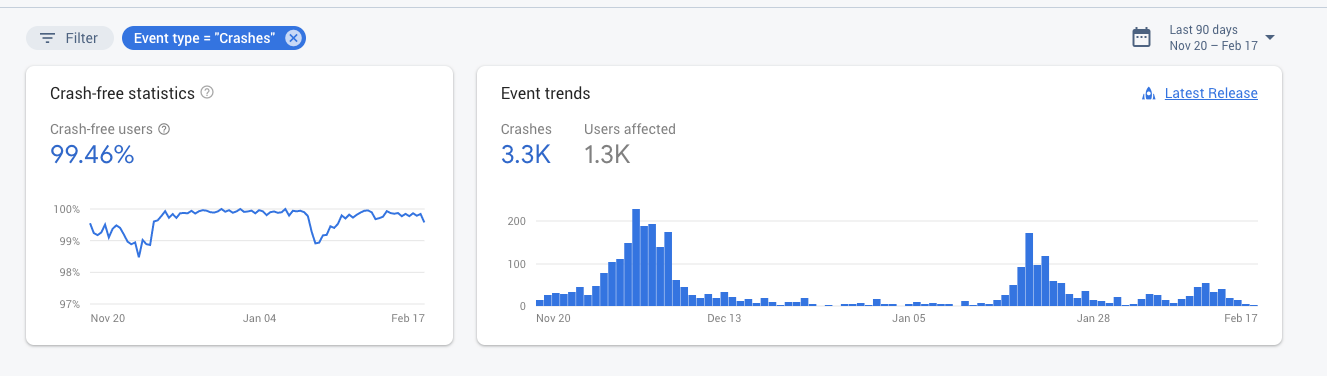
\includegraphics[width=14cm]{images/moonpig/firebase_crash_graph_90_days_feb_2020.png}} \\
    90 day view \\
    {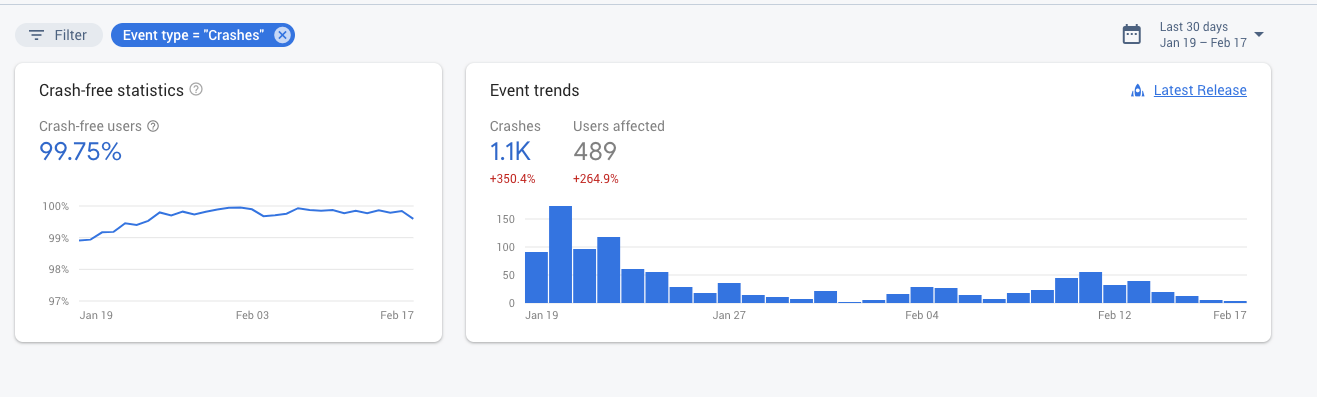
\includegraphics[width=14cm]{images/moonpig/firebase_crash_graph_30_days_17_feb_2020.png}} \\
    30 day view \\
    {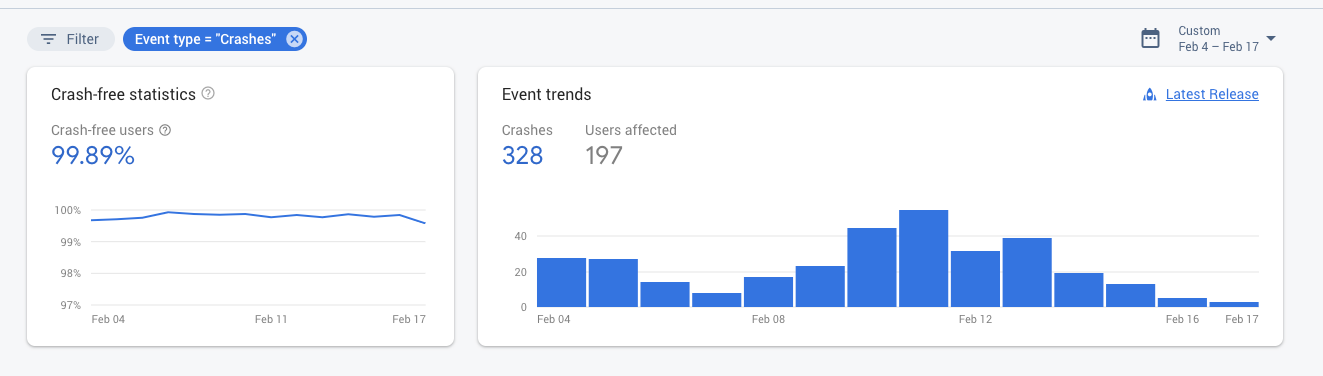
\includegraphics[width=14cm]{images/moonpig/firebase_crash_graph_14_days_feb_2020.png}} \\
    14 day view
    \end{tabular}
    \caption{Moonpig: Firebase Analytics crash free session graphs}
    \label{fig:moonpig-firebase-feb2020-crash-free-sessions}
\end{figure}




``The recent crash was introduced on the 10th Jan and the hotfix released on the 17th Jan [2020]." (the second crash)
``The previous one was introduced on the 25th Nov and the hotfix released on the 5th Dec [2019]." (the first crash)

The process Moonpig took from discovering the crash to addressing it and being ready to release the updated app.

How the first crash was addressed
\begin{quote}
    ``[It] was more straightforward to fix. I think it was a silly null pointer."
\end{quote}

How the second crash was addressed
\begin{quote}
    ``we noticed them by monitoring with Crashlytics/Firebase, I think specifically in the last case we got a crash velocity alert.

      The first thing we did was trying to find a way to reproduce the crash as it wasn't very clear what is happening. This took us a good chunk of a day. Once we knew where the issue came from we discussed different approaches to fixing it. 
      
      All of the initial ideas were more workarounds than a good solid fix. We discussed if we should push for a quick fix and investigate a better solution after that but decided against it as the crash "only" affected 1\% of our users. We spent another day finding a better way to fix it and in the end found a robust solution. We created automated tests that would result in the crash to make sure that we actually solved the problem.
      
      One day later we published a new release with the fix in. "
\end{quote} (email correspondence \nth{18} Feb 2020).

``The approach [to addressing crashes] is normally quite similar to what I've described though"



\newthought{Crashes mentioned in a user review}
\begin{wrapfigure}{R}{0.45\textwidth}
  %\begin{center}
    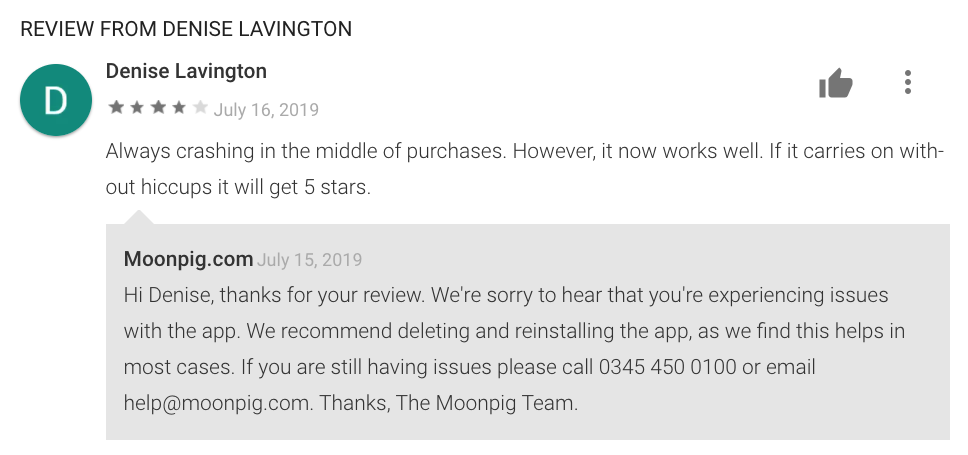
\includegraphics[width=0.44\textwidth]{images/google-play/Denise-Lavington-Review-moonpig-crashing-2019.png}
  %\end{center}
  \caption[Moonpig: User Review in Google Play `Always crashes...']{Moonpig: User Review `Always crashing in the middle of purchases'}
  \label{fig:gp-review-denise-lavington-always-crashes}
\end{wrapfigure}

On \nth{16} July 2019, Denise Lavington provided a review of the Android app and awarded the app four stars. The review said: \emph{``Always crashing in the middle of purchases. However, it now works well. If it carries on without hiccups it will get 5 stars."} Figure \ref{fig:gp-review-denise-lavington-always-crashes} shows the review in context in Google Play~\footnote{The review is currently still available online (\href{https://play.google.com/store/apps/details?id=com.commonagency.moonpig.uk&reviewId=gp\%3AAOqpTOH68VB5eWqnu7UAqcC81_rbOfWl6dzL_g48jrg0T40MPWBkMxe01KjStXZF6F57nxZxQa-AqosRKDd1xQ}{here}) in Google Play, two years after it was written.}.

The developer investigated this reported issue and could not find any crash in Firebase or Android Vitals that might affect purchases. A possible reason for why the crash did not appear in Android Vitals is that the underlying data is only provided by a user's device if they've opted-in to automatically providing their usage and diagnostics data~\citep{google_play_view_crashes_and_anr_errors} \textit{and} if the aggregate data exceeds an undocumented threshold (a topic discussed elsewhere in the thesis).

\subsection{Moonpig: data collected and methods used for collection}
The data was collected though a mix of in-person and online working sessions together with various email conversations. Screenshots and other materials were emailed by the developer to the researcher. 

The developer also ran Vitals Scraper to help evaluate whether it worked beyond the local use as part of various case studies. They sent the JSON results containing the crash clusters collected by Vitals Scraper.  

\subsection{Moonpig: Research findings and results from the Case Study}

\begin{figure}
    \centering
    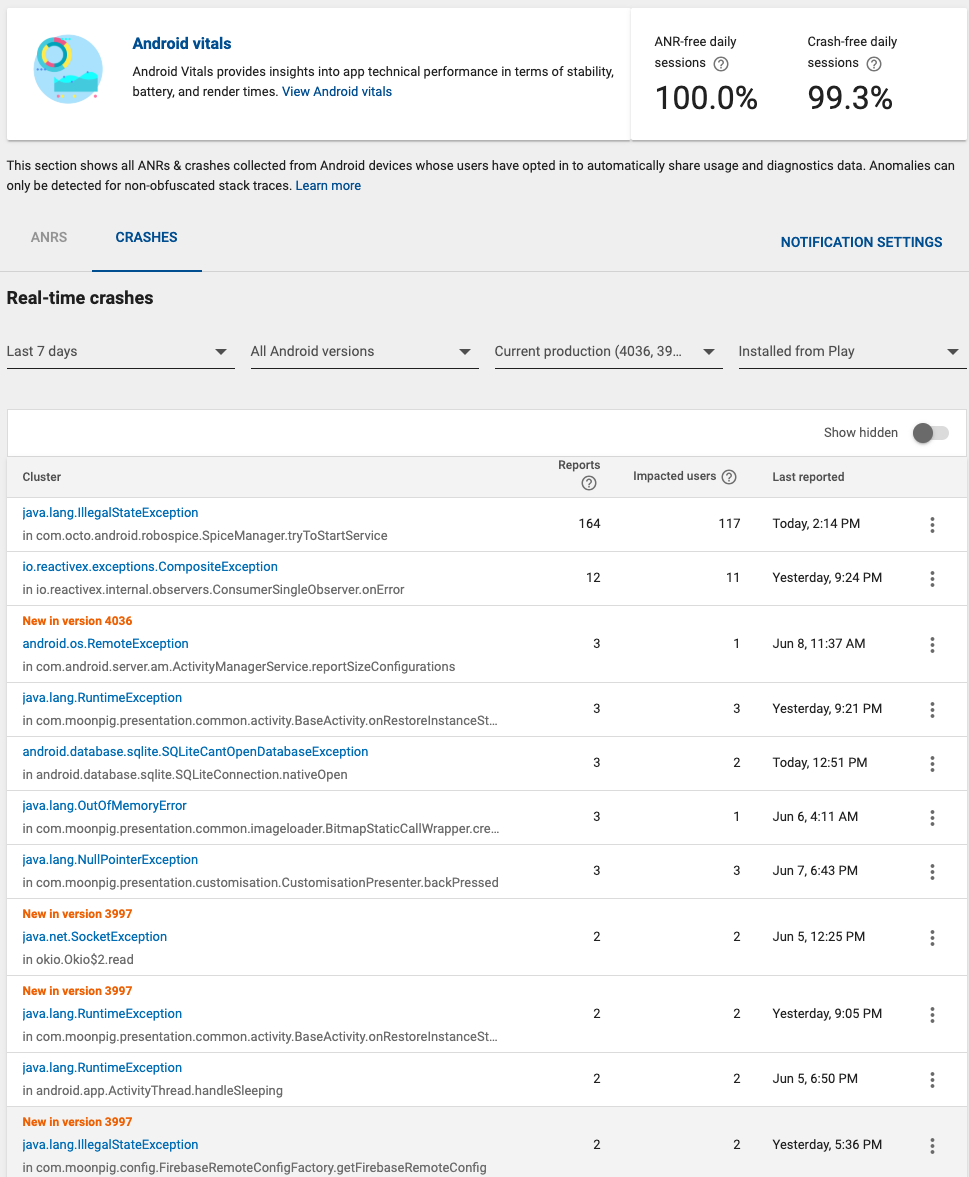
\includegraphics[width=12cm]{images/android-vitals-screenshots/moonpig/real-time-crashes-Screenshot-2019-06-10-at-15.42.34.png}
    \caption{Moonpig: Android Vitals snapshot of top crashes \nth{10} June 2019}
    \label{fig:av-moonpig-top-real-time-crashes-10-jun-2019}
\end{figure}

\begin{figure}
    \centering
    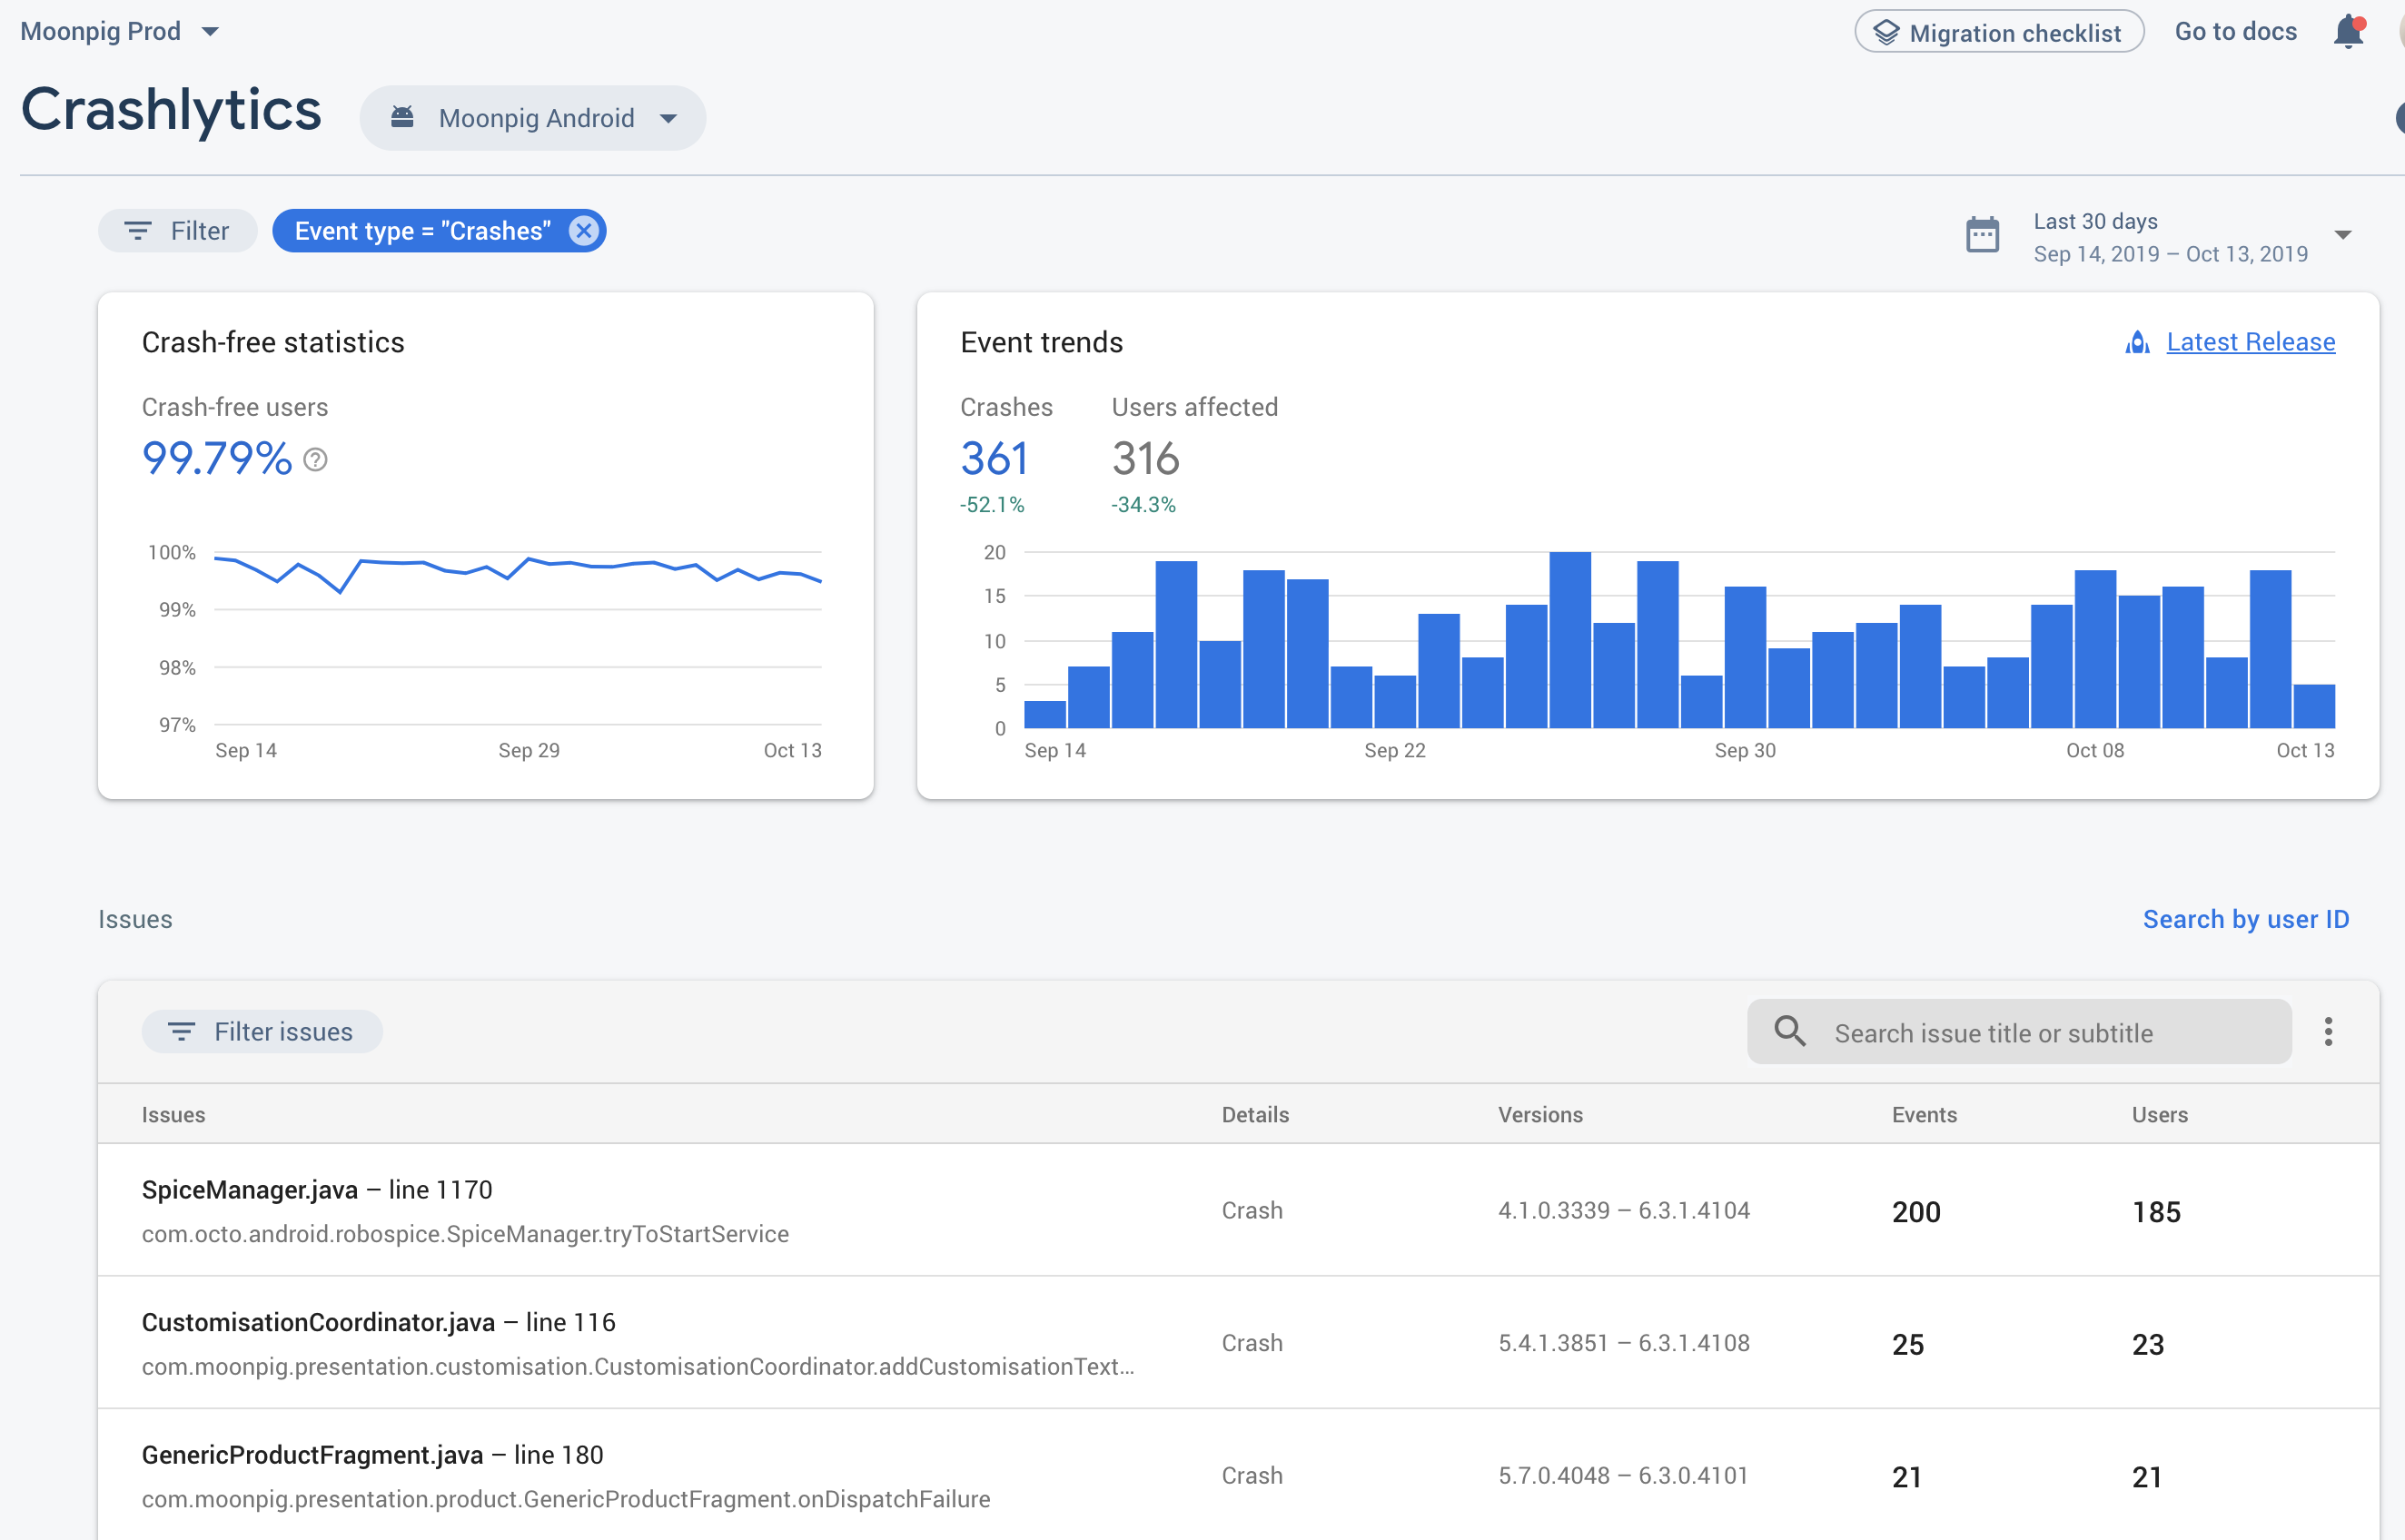
\includegraphics[width=12cm]{images/moonpig/Firebase-Crashlytics-30D-SpiceManagerCrashes.png}
    \caption{Moonpig: Firebase Crashlytics Spice Manager crashes}
    \label{fig:firebase-crashlytics-moonpig-spicemanager-crashes-30d}
\end{figure}

In Figure~\ref{fig:av-moonpig-top-real-time-crashes-10-jun-2019} Android Vitals shows the most frequent crash clusters for the production releases of the Moonpig Android app. The majority of crashes were an \texttt{IllegalStateException} in a third-party library SpiceManager, part of the RoboSpice opensource project \url{https://github.com/stephanenicolas/robospice}. 

This crash is an excellent example of how changes and new developments in the ecosystem can render what was reliable working software into software that is no longer fit for purpose, \emph{i.e.} RoboSpice was developed in 2012 to help developers simplify coding of asynchronous networking requests \url{https://github.com/stephanenicolas/robospice} and the library worked really well at the time and for several years afterwards. It became popular as a result and was used widely by many teams, including at Moonpig. However, as the Google Android platform morphed some of the changes to Android were incompatible with RoboSpice. And with Android Oreo (Release 8.0) changes to the way background services worked broke the functionality of the library sufficiently that the project was archived by the creator and project owner \url{https://github.com/stephanenicolas/robospice/issues/467} 

For apps that used RoboSpice the crash rate increased on the newer releases of Android, for example Figure~\ref{fig:av-moonpig-crash-rate-groupings} shows the crash rates by Android version were lowest on Android 7, higher for Android 8 and 8.1, and significantly higher again for Android 9. The teams needed to allocate time and energy to finding a suitable alternative to RoboSpice and then implement and test the new approach. In the interim the continued to `target' Android SDK 26 to mitigate the impact of running the app on devices running Android 9. Android Vitals helped provide an indication of the effects of the crashed and therefore provided evidence the development team could use to assess and prioritise the work.

\begin{figure}
    \centering
    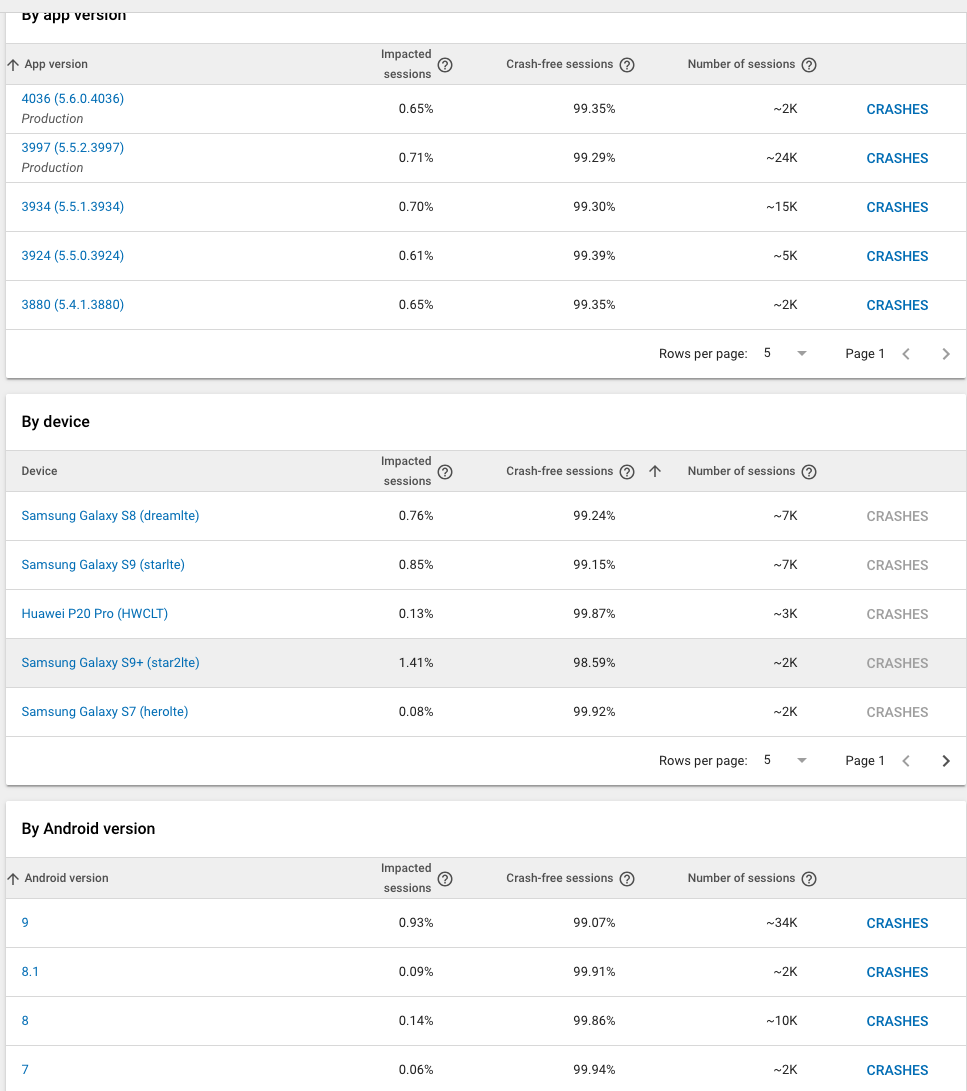
\includegraphics[width=13cm]{images/android-vitals-screenshots/moonpig/Screenshot 2019-06-10 at 15.41.23.png}
    \caption{Android Vitals: Moonpig various groupings of the crash rate \nth{10} June 2019}
    \label{fig:av-moonpig-crash-rate-groupings}
\end{figure}

\subsection{Moonpig: Outcomes for the company}
For over two years since the case study started, in June 2019, the Android app has been highly rated by end users in Google Play. According to AppBrain it is in the top 1\% of apps by rating, and in the top 5\% in both ratings (46,000) and downloads (estimated at 3,000,000)~\citep{appbrain_moonpig}.

The company was able to `go public' in February 2021 by listing on the London Stock Exchange.  

\subsection{Moonpig: Discussion}
The engineering team had integrated the use of mobile analytics into their development, engineering, and operational practices. They endeavoured to collect sufficient data to enable them to respond quickly to failures in use with their app and to analyse new issues within days so they could address the issues quickly, efficiently, and effectively. They were able to do so through incorporating Firebase Analytics in addition to Firebase Crashlytics. Firebase Analytics is discussed in more detail in \secref{chapter-discussion} and in \secref{appendix-analytics-tools}.

The nature of Moonpig's business means they often have information pertaining to users of their app: users need to be logged in to use the shopping basket and make purchases, \emph{etc.} 
Some of the bugs may pertain to user-specific data. Firebase is one of a wide range of mobile analytics offerings that can collect user-related data TODO...


Their privacy policy at the time~\citep{moonpig_privacy_policy_2019_feb_21}, and subsequently in~\citep{moonpig_privacy_policy_2021_aug_12} alludes to the the type of data being recorded, the purposes of collecting it, and who it may be shared with. Mobile Analytics is not mentioned explicitly, nor are the providers of the analytics services.



\subsection{Moonpig: Contributions to the research and where they are located in the rest of this thesis}
This case study provides contributions to the Findings section \secref{findings-section}. It also a source used when describing Firebase Analytics in \secref{chapter-discussion} and in \secref{appendix-analytics-tools}. It also supports Vitals Scraper, covered in \secref{section-vitals-scraper}. \secref{prerequisites-desirable}

%%% Ad-hoc notes from meeting Jakob D. Moonpig
% Business changes including the company's IPO mean the company has cut back on information they're willing to share internally and externally (e.g. for my PhD research).